\section{Context-sensitive visitor}
\label{sect:impl:context_sens_visitor}
In section \ref{sect:theory:parser:tree_parsing} a number of techniques for
tree parsing were presented. In section \ref{sect:method:tree_parsing} the
\textit{context-sensitive visitor pattern} was chosen as the technique for this
implementation. This section will detail the implementation of this design
pattern, and how it is used to performed an assortment of tasks.

\subsection{Basics}
The context-sensitive pattern is designed to be flexible and to generate code
with a higher level of maintainability, for which the rationale was presented
in section \ref{sect:theory:contextVisitorPattern}. 

\begin{figure}[htp]
\begin{center}
  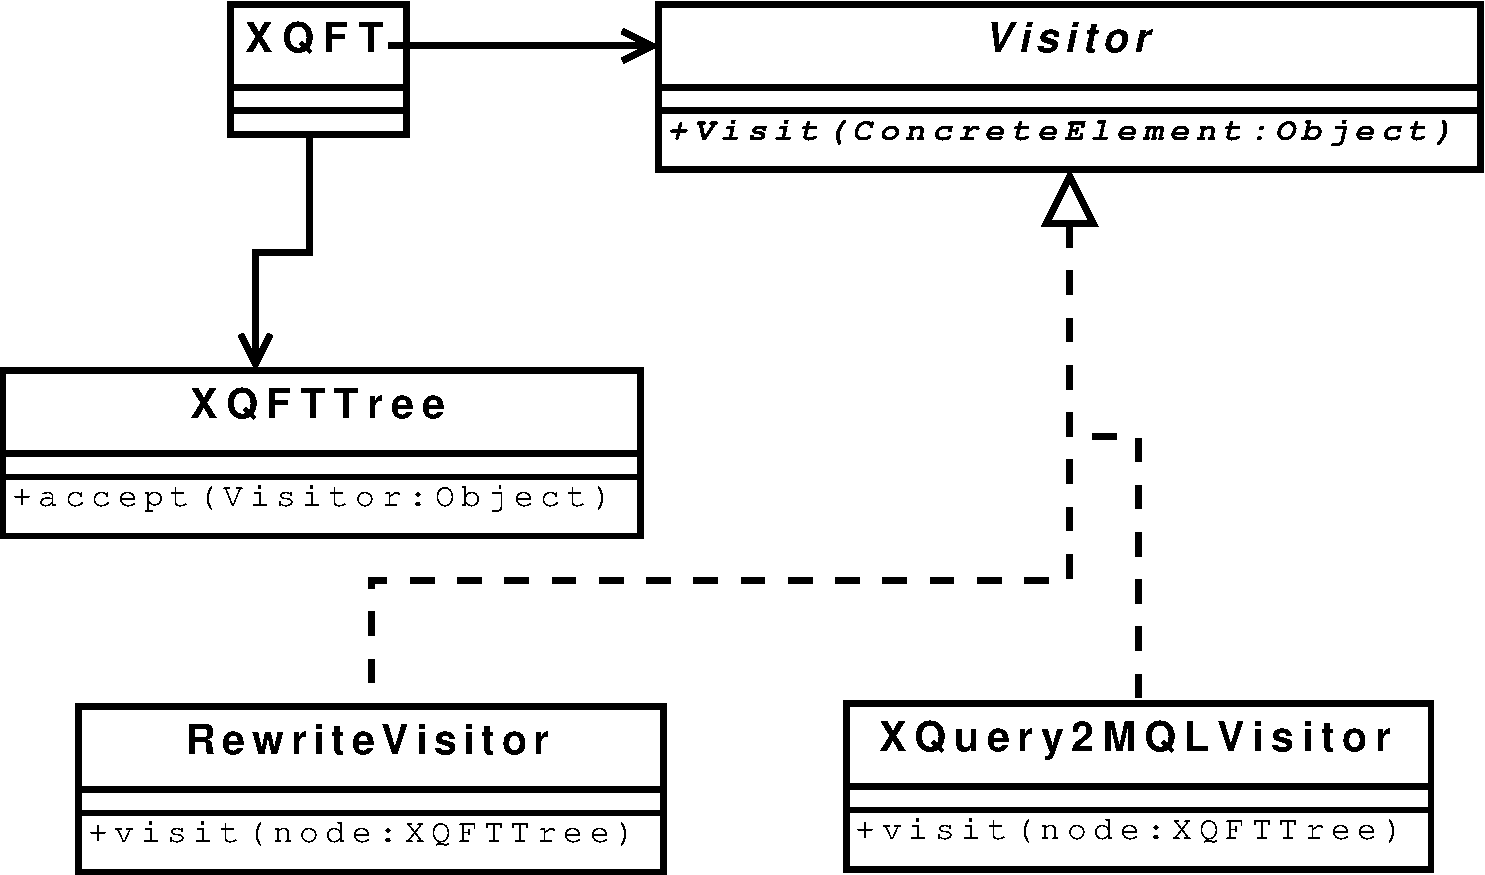
\includegraphics[scale=0.5]{diagrams/context_visitor_pattern_impl}
  \caption{Context sensitive visitor implementation}
  \label{fig:impl:context_sens_visitor_impl}
\end{center}
\end{figure}

TODO: herregud, dette diagrammet er litt feil.

The class diagram for the actual implementation of the context-sensitive
visitor pattern can be seen in figure \ref{fig:impl:context_sens_visitor_impl}.
Compare this to the generalized class diagram in figure
\ref{figure:parser:context_visitor_pattern} on page
\pageref{figure:parser:context_visitor_pattern}.

Note that the use of \texttt{XQFTTree} as the element class implies that the
\texttt{XQFTTree} be supplemented with an \texttt{accept()} method to
accommodate this pattern. This method is essentially a static dispatcher which
will call the appropriate method on the visitor based on the token type of the
node currently being visited. Figure \ref{} shows an excerpt of this method and
how it acts on the visitor class.

%\usepackage{graphics} is needed for \includegraphics
\begin{figure}[htp]
\begin{center}
  \begin{Verbatim}	
public TraverseReturn accept(Visitor visitor) {
     case XQFTParser.AST_MODULE:
            return visitor.visitAST_MODULE(this);
        case XQFTParser.AST_FLWOR:
            return visitor.visitAST_FLWOR(this);
        case XQFTParser.AST_FORCLAUSE:
            return visitor.visitAST_FORCLAUSE(this);
        case XQFTParser.AST_LETCLAUSE:
            return visitor.visitAST_LETCLAUSE(this);
        case XQFTParser.AST_ORDERBYCLAUSE:
            return visitor.visitAST_ORDERBYCLAUSE(this);
        case XQFTParser.AST_WHERECLAUSE:
            return visitor.visitAST_WHERECLAUSE(this);
                          .
                          .
                          .
  \end{Verbatim}
  \caption{Excerpt from the accept() method in the XQFT class}
  \label{figureLabel}
\end{center}
\end{figure}

\subsection{The Rewrite visitor}
The \textit{Rewrite visitor} is used to perform rewrite operations on the
abstract syntax tree before performing the actual translation. In particular,
these rewrite operations consists of normalizing the required subtrees of the
syntax tree to a subset of XQuery Core (as described in sections
\ref{sect:theory:xquery:XQcore} and \ref{sect:method:ast_rewrite}).

\subsection{The XQuery2MQL visitor}
The \textit{XQuery2MQL visitor} performs the bulk of the work related to
performing the translation of XQuery to MQL. This visitor is capable of
re-instantiating itself (or other visitors) when entering new contexts, such as
path predicates.

TODO: noe om TraverseReturn og hvordan MQL-treet blir bygd bottom-up